% GridTokenX White Paper - Simplified Version
% LaTeX Version 1.0 - December 2025
% Blockchain-Based P2P Energy Trading Platform
% Compatible with basic TeX Live installation

\documentclass[11pt,a4paper]{article}

% ============================================================================
% PACKAGES (Core packages available in basic TeX installations)
% ============================================================================
\usepackage[utf8]{inputenc}
\usepackage[T1]{fontenc}
\usepackage{lmodern}
\usepackage{geometry}
\usepackage{graphicx}
\usepackage{xcolor}
\usepackage{hyperref}
\usepackage{amsmath,amssymb}
\usepackage{booktabs}
\usepackage{tabularx}
\usepackage{longtable}
\usepackage{fancyhdr}
\usepackage{tikz}
\usepackage{pgfplots}
\usepackage{float}
\usepackage{listings}
\usepackage{caption}
\usepackage{multirow}
\usepackage{array}
\usepackage{setspace}
\usepackage{parskip}

% ============================================================================
% PAGE SETUP
% ============================================================================
\geometry{
    top=2.5cm,
    bottom=2.5cm,
    left=2.5cm,
    right=2.5cm,
    headheight=14pt
}

% ============================================================================
% COLORS
% ============================================================================
\definecolor{gridgreen}{RGB}{34, 139, 34}
\definecolor{gridblue}{RGB}{70, 130, 180}
\definecolor{griddark}{RGB}{45, 52, 54}
\definecolor{gridlight}{RGB}{236, 240, 241}
\definecolor{solana}{RGB}{153, 69, 255}
\definecolor{codegreen}{rgb}{0,0.6,0}
\definecolor{codegray}{rgb}{0.5,0.5,0.5}
\definecolor{codepurple}{rgb}{0.58,0,0.82}
\definecolor{backcolour}{rgb}{0.95,0.95,0.92}

% ============================================================================
% HYPERREF SETUP
% ============================================================================
\hypersetup{
    colorlinks=true,
    linkcolor=gridblue,
    filecolor=magenta,
    urlcolor=gridgreen,
    pdftitle={GridTokenX White Paper},
    pdfauthor={GridTokenX Team},
    pdfsubject={Blockchain-Based P2P Energy Trading Platform},
    pdfkeywords={blockchain, energy, trading, Solana, P2P, renewable energy}
}

% ============================================================================
% HEADER AND FOOTER
% ============================================================================
\pagestyle{fancy}
\fancyhf{}
\fancyhead[L]{\textcolor{griddark}{\textit{GridTokenX White Paper}}}
\fancyhead[R]{\textcolor{griddark}{\textit{Version 1.0}}}
\fancyfoot[C]{\thepage}
\renewcommand{\headrulewidth}{0.4pt}
\renewcommand{\footrulewidth}{0.4pt}

% ============================================================================
% CUSTOM BOX ENVIRONMENT (Simple version without tcolorbox)
% ============================================================================
\newenvironment{highlightbox}{%
    \begin{center}
    \begin{tabular}{|p{0.9\textwidth}|}
    \hline
    \rowcolor{gridlight}
}{%
    \\ \hline
    \end{tabular}
    \end{center}
}

\newenvironment{infobox}{%
    \begin{center}
    \begin{tabular}{|p{0.9\textwidth}|}
    \hline
    \rowcolor{blue!5}
}{%
    \\ \hline
    \end{tabular}
    \end{center}
}

\newenvironment{warningbox}{%
    \begin{center}
    \begin{tabular}{|p{0.9\textwidth}|}
    \hline
    \rowcolor{yellow!10}
}{%
    \\ \hline
    \end{tabular}
    \end{center}
}

% ============================================================================
% LISTING SETUP
% ============================================================================
\lstdefinestyle{mystyle}{
    backgroundcolor=\color{backcolour},
    commentstyle=\color{codegreen},
    keywordstyle=\color{magenta},
    numberstyle=\tiny\color{codegray},
    stringstyle=\color{codepurple},
    basicstyle=\ttfamily\footnotesize,
    breakatwhitespace=false,
    breaklines=true,
    captionpos=b,
    keepspaces=true,
    numbers=left,
    numbersep=5pt,
    showspaces=false,
    showstringspaces=false,
    showtabs=false,
    tabsize=2
}
\lstset{style=mystyle}

% ============================================================================
% TIKZ SETUP
% ============================================================================
\usetikzlibrary{shapes,arrows,positioning,calc,fit,backgrounds}
\pgfplotsset{compat=1.18}

% ============================================================================
% DOCUMENT START
% ============================================================================
\begin{document}

% ============================================================================
% TITLE PAGE
% ============================================================================
\begin{titlepage}
    \centering
    \vspace*{2cm}
    
    % Logo placeholder
    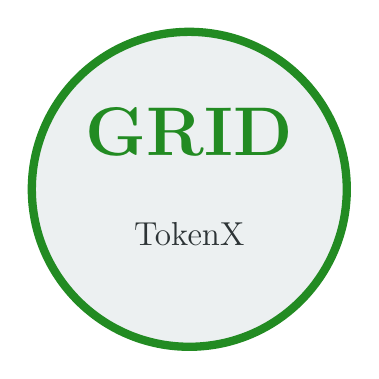
\begin{tikzpicture}
        \node[circle, draw=gridgreen, line width=3pt, minimum size=4cm, fill=gridlight] (logo) {};
        \node[above=0.3cm of logo.center, font=\Huge\bfseries, text=gridgreen] {GRID};
        \node[below=0.3cm of logo.center, font=\large, text=griddark] {TokenX};
    \end{tikzpicture}
    
    \vspace{2cm}
    
    {\Huge\bfseries\textcolor{griddark}{GridTokenX White Paper}}
    
    \vspace{0.5cm}
    
    {\Large\textcolor{gridblue}{Blockchain-Based P2P Energy Trading Platform}}
    
    \vspace{1cm}
    
    {\large\textcolor{griddark}{Decentralizing the Future of Energy}}
    
    \vspace{2cm}
    
    \fcolorbox{gridgreen}{gridlight}{%
        \parbox{0.8\textwidth}{%
            \centering
            \vspace{0.5cm}
            \textbf{\large 1 GRID Token = 1 kWh of Verified Renewable Energy}
            \vspace{0.5cm}
        }%
    }
    
    \vspace{2cm}
    
    \begin{tabular}{ll}
        \textbf{Version:} & 1.0 \\
        \textbf{Date:} & December 2025 \\
        \textbf{Status:} & Technical Specification \\
        \textbf{Blockchain:} & Solana \\
    \end{tabular}
    
    \vfill
    
    {\small\textcolor{codegray}{
        This document is for informational purposes only and does not constitute\\
        financial, legal, or investment advice. Please conduct your own research.
    }}
\end{titlepage}

% ============================================================================
% TABLE OF CONTENTS
% ============================================================================
\newpage
\tableofcontents
\newpage

% ============================================================================
% ABSTRACT
% ============================================================================
\section*{Abstract}
\addcontentsline{toc}{section}{Abstract}

The global energy landscape is undergoing a paradigm shift from centralized fossil-fuel generation to decentralized renewable energy resources (DERs). However, legacy grid infrastructure and centralized market mechanisms struggle to accommodate the bidirectional flow of energy and value required by this transition.

\textbf{GridTokenX} introduces a decentralized, peer-to-peer (P2P) energy trading platform built on the \textbf{Solana blockchain}. By tokenizing energy generation into \textbf{GRID tokens} (1 GRID = 1 kWh) and leveraging high-performance smart contracts, GridTokenX enables prosumers to trade excess energy directly with neighbors, ensuring fair pricing, instant settlement, and transparent provenance.

\vspace{0.5cm}
\fcolorbox{gridblue}{blue!5}{%
    \parbox{0.9\textwidth}{%
        \textbf{Key Innovation:} GridTokenX creates a trustless, automated marketplace where every kilowatt-hour of renewable energy is cryptographically verified, tokenized, and tradeable in real-time.
    }%
}
\vspace{0.5cm}

This paper outlines the technical architecture, economic model, security framework, and governance structure of the GridTokenX ecosystem.

% ============================================================================
% SECTION 1: INTRODUCTION
% ============================================================================
\section{Introduction}

\subsection{The Energy Transition}

The rapid adoption of solar photovoltaics (PV), battery storage, and electric vehicles has transformed traditional energy consumers into ``prosumers''---active participants who both consume and produce energy. According to the International Energy Agency (IEA), distributed solar capacity is expected to exceed 1,500 GW by 2030, representing a fundamental shift in how energy is generated and consumed.

While technology has advanced significantly, the market structure remains archaic, creating a gap between what is technologically possible and what the current infrastructure supports.

\subsection{Market Inefficiencies}

Current energy markets suffer from several fundamental challenges:

\begin{table}[H]
\centering
\caption{Traditional Energy Market Problems}
\begin{tabularx}{\textwidth}{lX}
\toprule
\textbf{Problem} & \textbf{Description} \\
\midrule
Centralized Intermediaries & Utility companies act as gatekeepers, setting buy/sell prices with significant spreads (typically 40-60\% markup). \\
\addlinespace
Lack of Transparency & Consumers have no visibility into the source of their energy (renewable vs. fossil fuel). \\
\addlinespace
Settlement Delays & Payments to producers often take weeks or months due to manual reconciliation processes. \\
\addlinespace
Data Silos & Smart meter data is locked within utility databases, preventing innovation and limiting consumer choice. \\
\addlinespace
Limited Price Discovery & No mechanism exists for true P2P price discovery in retail energy markets. \\
\bottomrule
\end{tabularx}
\end{table}

\subsection{Impact on Renewable Energy Adoption}

These inefficiencies create significant barriers to renewable energy adoption:

\begin{itemize}
    \item \textbf{Economic Barriers:} High installation costs, long payback periods, limited monetization options, and unfavorable feed-in tariffs.
    \item \textbf{Technical Barriers:} Grid connection complexity, intermittent generation challenges, storage requirements, and inadequate metering infrastructure.
    \item \textbf{Result:} Slower adoption of Distributed Energy Resources (DERs) than technologically feasible.
\end{itemize}

% ============================================================================
% SECTION 2: THE GRIDTOKENX SOLUTION
% ============================================================================
\section{The GridTokenX Solution}

GridTokenX addresses these challenges through a comprehensive blockchain-based P2P energy trading platform.

\subsection{Key Value Propositions}

\fcolorbox{gridgreen}{gridlight}{%
    \parbox{0.9\textwidth}{%
        \begin{enumerate}
            \item \textbf{Direct P2P Trading:} Prosumers sell excess energy directly to consumers at mutually agreed prices, eliminating intermediary markups.
            \item \textbf{Real-Time Settlement:} Blockchain transactions settle in seconds, not months.
            \item \textbf{Proof of Origin:} Every GRID token is cryptographically tied to a specific generation event, guaranteeing green energy provenance.
            \item \textbf{Automated Compliance:} Smart contracts enforce grid constraints and regulatory rules automatically.
        \end{enumerate}
    }%
}

\subsection{Platform Overview}

GridTokenX creates a trustless, automated marketplace by combining:

\begin{itemize}
    \item \textbf{Solana Blockchain:} High-throughput, low-cost infrastructure capable of handling micro-transactions.
    \item \textbf{Smart Meter Integration:} Real-time energy data feeds from verified IoT devices.
    \item \textbf{SPL Token Standard:} Fungible tokens representing verified energy production.
    \item \textbf{On-Chain Order Book:} Transparent price discovery and automated matching.
\end{itemize}

\subsection{The Dual-Tracker Model}

To satisfy both physical grid physics and financial markets, GridTokenX employs a dual-layer approach:

\begin{figure}[H]
\centering
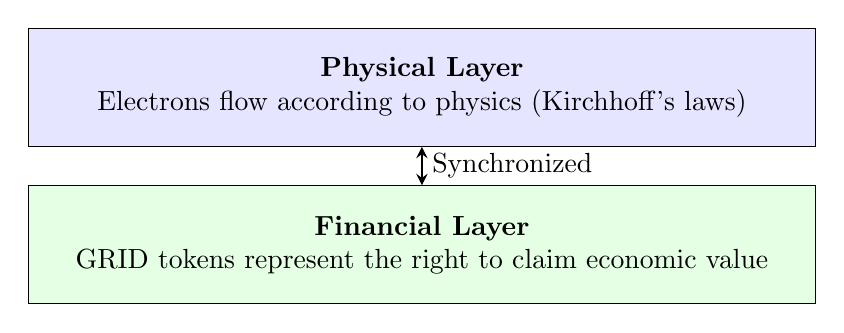
\begin{tikzpicture}[
    layer/.style={rectangle, draw, minimum width=10cm, minimum height=1.5cm, align=center},
    arrow/.style={->, thick, >=stealth}
]
    % Physical Layer
    \node[layer, fill=blue!10] (physical) at (0,2) {
        \textbf{Physical Layer}\\
        Electrons flow according to physics (Kirchhoff's laws)
    };
    
    % Financial Layer
    \node[layer, fill=green!10] (financial) at (0,0) {
        \textbf{Financial Layer}\\
        GRID tokens represent the right to claim economic value
    };
    
    % Arrows
    \draw[arrow, <->] (physical.south) -- (financial.north) node[midway, right] {Synchronized};
\end{tikzpicture}
\caption{GridTokenX Dual-Tracker Model}
\end{figure}

% ============================================================================
% SECTION 3: TECHNICAL ARCHITECTURE
% ============================================================================
\section{Technical Architecture}

\subsection{Blockchain Selection: Solana}

GridTokenX is built on \textbf{Solana}, chosen for its exceptional performance characteristics essential for energy micro-transactions:

\begin{table}[H]
\centering
\caption{Solana Performance Characteristics}
\begin{tabular}{lc}
\toprule
\textbf{Metric} & \textbf{Value} \\
\midrule
Theoretical TPS & 65,000+ \\
Block Time & 400ms \\
Average Transaction Cost & \$0.00025 \\
Finality & Sub-second \\
Consensus & Proof of History (PoH) + PoS \\
\bottomrule
\end{tabular}
\end{table}

\subsection{Core Smart Contract Programs}

The platform consists of five interacting Anchor programs written in Rust:

\subsubsection{Registry Program}

The Registry Program manages identity and access control for all platform participants.

\begin{lstlisting}[caption={Registry Program Structure}]
pub struct ProsumerConfig {
    pub owner: Pubkey,        // Wallet owner
    pub is_verified: bool,    // KYC status
    pub meter_id: Pubkey,     // Linked smart meter
    pub role: UserRole,       // Prosumer/Consumer/Verifier
    pub created_at: i64,      // Registration timestamp
}

pub enum UserRole {
    Prosumer,   // Can sell energy
    Consumer,   // Can buy energy
    Verifier,   // Can verify meters
    Admin,      // Platform administrator
}
\end{lstlisting}

\textbf{Key Functions:}
\begin{itemize}
    \item \texttt{register\_user} --- Create new user account with role assignment
    \item \texttt{verify\_meter} --- Link and verify smart meter device
    \item \texttt{update\_status} --- Modify user verification status
\end{itemize}

\subsubsection{Energy Token Program}

Implements the GRID SPL Token with Program Derived Address (PDA) authorities for trustless minting.

\begin{lstlisting}[caption={Token Minting Logic}]
pub fn mint_energy_tokens(
    ctx: Context<MintTokens>,
    meter_reading: MeterReading,
) -> Result<()> {
    // Verify meter reading signature
    require!(
        verify_oracle_signature(&meter_reading),
        ErrorCode::InvalidSignature
    );
    
    // Calculate tokens: 1 kWh = 1 GRID
    let amount = meter_reading.kwh_produced * DECIMALS;
    
    // Mint to prosumer's account
    token::mint_to(
        ctx.accounts.mint_to_ctx(),
        amount,
    )?;
    
    emit!(TokensMinted {
        prosumer: ctx.accounts.prosumer.key(),
        amount,
        meter_id: meter_reading.meter_id,
    });
    
    Ok(())
}
\end{lstlisting}

\subsubsection{Oracle Program}

The Oracle Program acts as the bridge between physical smart meters and the blockchain.

\begin{itemize}
    \item Validates meter readings and posts signed data on-chain
    \item Prevents data tampering through cryptographic signatures
    \item Maintains price feeds for market operations
    \item Ensures ``Garbage In, Garbage Out'' protection
\end{itemize}

\subsubsection{Trading Program}

Implements an on-chain order book for energy markets with full atomic settlement.

\begin{table}[H]
\centering
\caption{Trading Program Order Types}
\begin{tabular}{lp{8cm}}
\toprule
\textbf{Order Type} & \textbf{Description} \\
\midrule
Limit Ask & Sell GRID tokens at specified minimum price \\
Limit Bid & Buy GRID tokens at specified maximum price \\
Market Order & Execute immediately at best available price \\
\bottomrule
\end{tabular}
\end{table}

\begin{lstlisting}[caption={Order Matching Algorithm}]
pub fn match_orders(
    ctx: Context<MatchOrders>,
    order_id: u64,
) -> Result<()> {
    let ask = &ctx.accounts.ask_order;
    let bid = &ctx.accounts.bid_order;
    
    // Price matching: bid >= ask
    require!(
        bid.price_per_grid >= ask.price_per_grid,
        ErrorCode::PriceMismatch
    );
    
    // Calculate settlement
    let quantity = min(ask.quantity, bid.quantity);
    let settlement_price = ask.price_per_grid; // Maker price
    
    // Atomic swap: GRID <-> Payment
    transfer_grid_tokens(&ctx, quantity)?;
    transfer_payment(&ctx, quantity * settlement_price)?;
    
    Ok(())
}
\end{lstlisting}

\subsubsection{Governance Program}

Enables decentralized decision-making through stake-weighted voting.

\begin{itemize}
    \item \textbf{Proposal Creation:} Stakeholders submit protocol change proposals
    \item \textbf{Voting Mechanism:} Token-weighted voting with configurable quorum
    \item \textbf{Execution:} Approved proposals execute automatically via CPI
\end{itemize}

\subsection{System Architecture Diagram}

\begin{figure}[H]
\centering
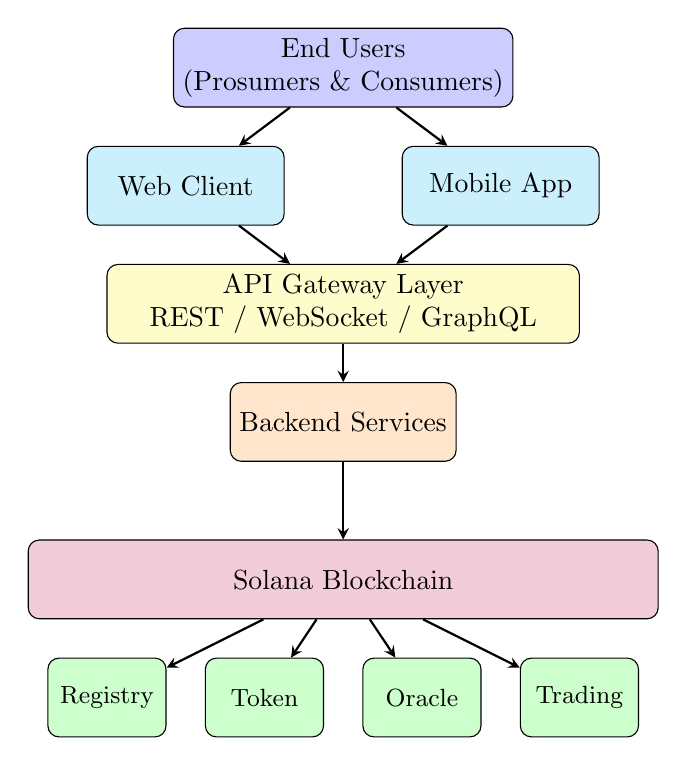
\begin{tikzpicture}[
    block/.style={rectangle, draw, minimum width=2.5cm, minimum height=1cm, align=center, rounded corners},
    arrow/.style={->, thick, >=stealth}
]
    % User Layer
    \node[block, fill=blue!20] (users) at (0,6) {End Users\\(Prosumers \& Consumers)};
    
    % Frontend Layer
    \node[block, fill=cyan!20] (web) at (-2,4.5) {Web Client};
    \node[block, fill=cyan!20] (mobile) at (2,4.5) {Mobile App};
    
    % API Layer
    \node[block, fill=yellow!20, minimum width=6cm] (api) at (0,3) {API Gateway Layer\\REST / WebSocket / GraphQL};
    
    % Backend Layer
    \node[block, fill=orange!20] (backend) at (0,1.5) {Backend Services};
    
    % Blockchain Layer
    \node[block, fill=purple!20, minimum width=8cm] (solana) at (0,-0.5) {Solana Blockchain};
    
    % Programs
    \node[block, fill=green!20, minimum width=1.5cm, font=\small] (registry) at (-3,-2) {Registry};
    \node[block, fill=green!20, minimum width=1.5cm, font=\small] (token) at (-1,-2) {Token};
    \node[block, fill=green!20, minimum width=1.5cm, font=\small] (oracle) at (1,-2) {Oracle};
    \node[block, fill=green!20, minimum width=1.5cm, font=\small] (trading) at (3,-2) {Trading};
    
    % Arrows
    \draw[arrow] (users) -- (web);
    \draw[arrow] (users) -- (mobile);
    \draw[arrow] (web) -- (api);
    \draw[arrow] (mobile) -- (api);
    \draw[arrow] (api) -- (backend);
    \draw[arrow] (backend) -- (solana);
    \draw[arrow] (solana) -- (registry);
    \draw[arrow] (solana) -- (token);
    \draw[arrow] (solana) -- (oracle);
    \draw[arrow] (solana) -- (trading);
\end{tikzpicture}
\caption{GridTokenX System Architecture}
\end{figure}

% ============================================================================
% SECTION 4: TOKEN ECONOMICS
% ============================================================================
\section{Token Economics}

\subsection{GRID Token Specification}

\begin{table}[H]
\centering
\caption{GRID Token Technical Specification}
\begin{tabular}{ll}
\toprule
\textbf{Property} & \textbf{Value} \\
\midrule
Token Name & GridTokenX Energy Token \\
Symbol & GRID \\
Standard & SPL Token (Solana Program Library) \\
Decimals & 9 \\
Supply Type & Elastic (Mint/Burn based on energy) \\
\midrule
\multicolumn{2}{c}{\textbf{Backing}} \\
\midrule
Peg & 1 GRID = 1 kWh of Verified Renewable Energy \\
Mint Authority & Energy Token Program PDA \\
Freeze Authority & None (freely transferable) \\
Burn Authority & Token holder + Program \\
\bottomrule
\end{tabular}
\end{table}

\subsection{Token Value Components}

The GRID token derives value from three key components:

\begin{enumerate}
    \item \textbf{Intrinsic Value:} Backed by verified energy production (1 kWh physical energy)
    \item \textbf{Utility Value:} Required for P2P trading on the platform; enables fee discounts
    \item \textbf{Scarcity Value:} Supply tied to actual production; no arbitrary minting
\end{enumerate}

\subsection{Elastic Supply Mechanism}

\begin{figure}[H]
\centering
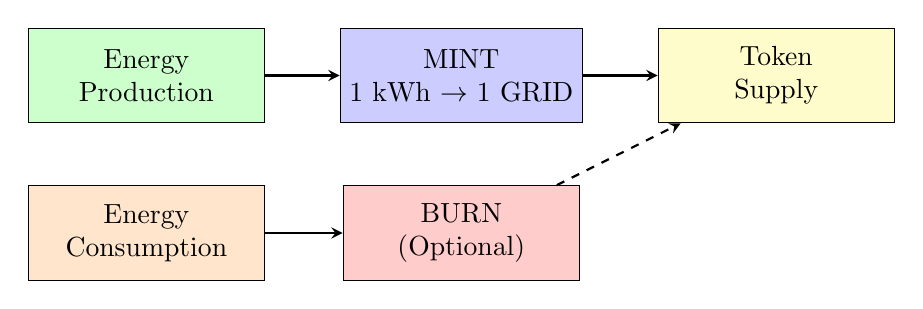
\begin{tikzpicture}[
    process/.style={rectangle, draw, minimum width=3cm, minimum height=1.2cm, align=center},
    arrow/.style={->, thick, >=stealth}
]
    % Production side
    \node[process, fill=green!20] (produce) at (-4,0) {Energy\\Production};
    \node[process, fill=blue!20] (mint) at (0,0) {MINT\\1 kWh $\rightarrow$ 1 GRID};
    \node[process, fill=yellow!20] (supply) at (4,0) {Token\\Supply};
    
    % Consumption side
    \node[process, fill=orange!20] (consume) at (-4,-2) {Energy\\Consumption};
    \node[process, fill=red!20] (burn) at (0,-2) {BURN\\(Optional)};
    
    % Arrows
    \draw[arrow] (produce) -- (mint);
    \draw[arrow] (mint) -- (supply);
    \draw[arrow] (consume) -- (burn);
    \draw[arrow, dashed] (burn) -- (supply);
\end{tikzpicture}
\caption{Elastic Supply Mechanism}
\end{figure}

\begin{equation}
\text{Total Supply} = \sum \text{Minted} - \sum \text{Burned}
\end{equation}

\subsection{Token Lifecycle}

\begin{enumerate}
    \item \textbf{Generation:} Solar panel produces 10 kWh. Smart meter signs data.
    \item \textbf{Minting:} Oracle validates data; Energy Token Program mints 10 GRID to prosumer.
    \item \textbf{Trading:} Prosumer lists 10 GRID on the Trading Program. Consumer buys them with USDC/SOL.
    \item \textbf{Settlement:} Consumer ``redeems'' GRID tokens against their consumption. Tokens optionally burned.
\end{enumerate}

\subsection{Supply Growth Projection}

\begin{table}[H]
\centering
\caption{Projected Token Supply Growth}
\begin{tabular}{lccc}
\toprule
\textbf{Quarter} & \textbf{Prosumers} & \textbf{Monthly Mint} & \textbf{Cumulative Supply} \\
\midrule
Year 1 Q1 & 100 & 50,000 GRID & 150,000 GRID \\
Year 1 Q2 & 125 & 62,500 GRID & 337,500 GRID \\
Year 1 Q3 & 156 & 78,000 GRID & 571,500 GRID \\
Year 1 Q4 & 195 & 97,500 GRID & 864,000 GRID \\
Year 2 Q1 & 244 & 122,000 GRID & 1,230,000 GRID \\
Year 2 Q2 & 305 & 152,500 GRID & 1,687,500 GRID \\
\bottomrule
\end{tabular}

\small\textit{Assumptions: 25\% quarterly growth, 500 kWh/month average surplus per prosumer}
\end{table}

\subsection{Economic Incentives}

\begin{itemize}
    \item \textbf{Prosumers:} Earn 15-30\% higher rates than utility feed-in tariffs
    \item \textbf{Consumers:} Pay 10-20\% lower rates than standard grid prices
    \item \textbf{Platform:} 0.25-0.5\% transaction fee funds protocol maintenance and DAO treasury
\end{itemize}

% ============================================================================
% SECTION 5: SECURITY FRAMEWORK
% ============================================================================
\section{Security Framework}

\subsection{Security Design Principles}

GridTokenX implements a defense-in-depth security strategy based on:

\begin{enumerate}
    \item \textbf{Least Privilege:} Grant only minimum necessary permissions to each component
    \item \textbf{Fail Secure:} Default to secure state on errors or unexpected conditions
    \item \textbf{Zero Trust:} Verify everything, trust nothing; authenticate all requests
\end{enumerate}

\subsection{Threat Model (STRIDE Analysis)}

\begin{table}[H]
\centering
\caption{STRIDE Threat Analysis}
\begin{tabularx}{\textwidth}{lXl}
\toprule
\textbf{Threat} & \textbf{Description} & \textbf{Mitigation} \\
\midrule
Spoofing & Impersonating another entity & Ed25519 signatures, PKI \\
Tampering & Unauthorized data modification & Immutable blockchain state \\
Repudiation & Denying actions performed & On-chain audit trail \\
Info Disclosure & Exposing sensitive data & Encryption, access controls \\
Denial of Service & Service unavailability & Rate limiting, redundancy \\
Elevation of Privilege & Unauthorized access & Role-based access control \\
\bottomrule
\end{tabularx}
\end{table}

\subsection{Smart Contract Security}

\fcolorbox{orange}{yellow!10}{%
    \parbox{0.9\textwidth}{%
        \textbf{Security Measures Implemented:}
        \begin{itemize}
            \item All programs undergo third-party security audits before mainnet deployment
            \item Reentrancy guards on all state-modifying functions
            \item Integer overflow/underflow protection via checked math
            \item Access control through PDA-based authority patterns
            \item Comprehensive test coverage ($>$95\%) including fuzz testing
        \end{itemize}
    }%
}

\subsection{Oracle Security}

The Oracle Program implements multiple layers of protection:

\begin{enumerate}
    \item \textbf{Multi-Signature Verification:} Meter readings require multiple oracle signatures
    \item \textbf{Staleness Checks:} Data older than configurable threshold is rejected
    \item \textbf{Deviation Bounds:} Abnormal readings trigger manual review
    \item \textbf{Slashing Mechanism:} Malicious oracles lose staked collateral
\end{enumerate}

% ============================================================================
% SECTION 6: GOVERNANCE
% ============================================================================
\section{Governance and DAO}

GridTokenX is designed to evolve into a fully Decentralized Autonomous Organization (DAO).

\subsection{Governance Phases}

\begin{table}[H]
\centering
\caption{Governance Evolution Roadmap}
\begin{tabular}{lp{6cm}l}
\toprule
\textbf{Phase} & \textbf{Description} & \textbf{Timeline} \\
\midrule
Phase 1: Federated & Core team and partners manage Registry and Oracle nodes & 2025 \\
Phase 2: Community & Token holders vote on fee structures and protocol upgrades & 2026 \\
Phase 3: Full DAO & Automated algorithmic governance of all parameters & 2027+ \\
\bottomrule
\end{tabular}
\end{table}

\subsection{Voting Mechanism}

\begin{itemize}
    \item \textbf{Proposal Threshold:} Minimum 1,000 GRID tokens to submit proposal
    \item \textbf{Voting Period:} 7 days for standard proposals, 3 days for emergency
    \item \textbf{Quorum:} 10\% of circulating supply must participate
    \item \textbf{Approval:} 66\% supermajority required for protocol changes
\end{itemize}

\subsection{Governable Parameters}

The following parameters can be modified through governance:

\begin{enumerate}
    \item Trading fee percentages (0.1\% -- 1.0\%)
    \item Minimum/maximum order sizes
    \item Oracle data staleness thresholds
    \item New program deployments and upgrades
    \item Treasury fund allocation
\end{enumerate}

% ============================================================================
% SECTION 7: COMPARATIVE ANALYSIS
% ============================================================================
\section{Comparative Analysis}

\subsection{Platform Comparison}

\begin{table}[H]
\centering
\caption{GridTokenX vs. Existing Platforms}
\resizebox{\textwidth}{!}{
\begin{tabular}{lccccc}
\toprule
\textbf{Feature} & \textbf{GridTokenX} & \textbf{Power Ledger} & \textbf{Energy Web} & \textbf{WePower} & \textbf{Traditional} \\
\midrule
Blockchain & Solana & Custom & EW Chain & Ethereum & N/A \\
TPS Capacity & 65,000+ & 1,000 & 500 & 15-30 & N/A \\
Transaction Cost & \$0.00025 & \$0.01 & \$0.001 & \$2-20 & \$1-5 \\
Settlement Time & Seconds & Minutes & Minutes & Minutes & Days-Months \\
P2P Trading & \checkmark & \checkmark & \checkmark & Limited & $\times$ \\
Smart Meter Integration & Native & Partner & Partner & Limited & Utility \\
Green Certification & On-chain & On-chain & On-chain & On-chain & Manual \\
\bottomrule
\end{tabular}
}
\end{table}

\subsection{Key Differentiators}

\fcolorbox{gridgreen}{gridlight}{%
    \parbox{0.9\textwidth}{%
        \textbf{GridTokenX Unique Advantages:}
        \begin{enumerate}
            \item \textbf{Highest Throughput:} Solana enables true micro-transaction economics
            \item \textbf{Lowest Costs:} Sub-cent transaction fees make small trades viable
            \item \textbf{Native Smart Meter Integration:} Purpose-built oracle system for energy data
            \item \textbf{Southeast Asia Focus:} Optimized for Thai/ASEAN regulatory environment
        \end{enumerate}
    }%
}

% ============================================================================
% SECTION 8: ROADMAP
% ============================================================================
\section{Roadmap}

\subsection{Development Timeline}

\begin{figure}[H]
\centering
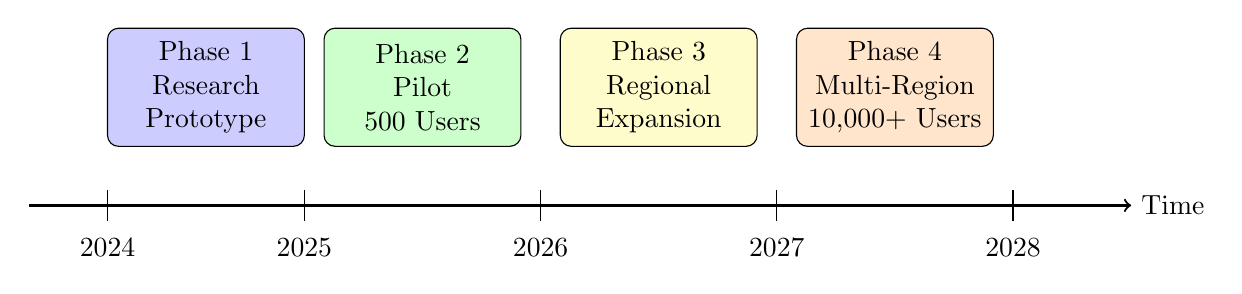
\begin{tikzpicture}[
    phase/.style={rectangle, draw, minimum width=2.5cm, minimum height=1.5cm, align=center, rounded corners},
    arrow/.style={->, thick, >=stealth}
]
    % Timeline
    \draw[thick, ->] (0,0) -- (14,0) node[right] {Time};
    
    % Phase markers
    \foreach \x/\year in {1/2024, 3.5/2025, 6.5/2026, 9.5/2027, 12.5/2028} {
        \draw (\x,-0.2) -- (\x,0.2);
        \node[below] at (\x,-0.3) {\year};
    }
    
    % Phases
    \node[phase, fill=blue!20] at (2.25,1.5) {Phase 1\\Research\\Prototype};
    \node[phase, fill=green!20] at (5,1.5) {Phase 2\\Pilot\\500 Users};
    \node[phase, fill=yellow!20] at (8,1.5) {Phase 3\\Regional\\Expansion};
    \node[phase, fill=orange!20] at (11,1.5) {Phase 4\\Multi-Region\\10,000+ Users};
\end{tikzpicture}
\caption{GridTokenX Development Roadmap}
\end{figure}

\subsection{Milestone Details}

\begin{table}[H]
\centering
\caption{Detailed Roadmap Milestones}
\begin{tabular}{llp{8cm}}
\toprule
\textbf{Quarter} & \textbf{Phase} & \textbf{Deliverables} \\
\midrule
Q1 2025 & 1 & Testnet Launch, Smart Contract Audits Complete \\
Q2 2025 & 2 & Pilot Program Launch (500 households, Bangkok) \\
Q3 2025 & 2 & Mainnet Beta Launch, Mobile App Release \\
Q4 2025 & 2 & Industrial Microgrid Integration \\
Q1 2026 & 3 & Regional Expansion (Thailand nationwide) \\
Q2 2026 & 3 & Carbon Credit Bridging Integration \\
Q3 2026 & 3 & ASEAN Market Entry (Vietnam, Indonesia) \\
Q4 2026 & 3 & Full DAO Governance Launch \\
\bottomrule
\end{tabular}
\end{table}

\subsection{Strategic Goals by 2028}

\begin{enumerate}
    \item \textbf{Technology Leadership:} Reference implementation for blockchain energy trading
    \item \textbf{Ecosystem Growth:} 100,000+ active users, 50+ partner integrations
    \item \textbf{Regulatory Compliance:} Full licenses in 3+ markets, ISO 27001 \& SOC2 certified
    \item \textbf{Sustainability Impact:} 1 TWh annual energy traded, 500,000 tons CO2 offset facilitated
\end{enumerate}

% ============================================================================
% SECTION 9: CONCLUSION
% ============================================================================
\section{Conclusion}

GridTokenX represents a critical infrastructure layer for the future of energy. By combining the immutable trust of blockchain technology with the efficiency of peer-to-peer markets, we are building an energy grid that is not only cleaner and more reliable but also economically empowering for every participant.

\fcolorbox{gridgreen}{gridlight}{%
    \parbox{0.9\textwidth}{%
        \textbf{Summary of Key Innovations:}
        \begin{itemize}
            \item \textbf{Tokenized Energy:} 1 GRID = 1 kWh, backed by verified renewable production
            \item \textbf{High-Performance Infrastructure:} Solana enables true micro-transaction economics
            \item \textbf{Trustless Verification:} Oracle-validated smart meter data ensures integrity
            \item \textbf{Decentralized Governance:} Community-driven protocol evolution
            \item \textbf{Economic Alignment:} All stakeholders benefit from platform growth
        \end{itemize}
    }%
}

\vspace{1cm}
The transition to renewable energy is inevitable. GridTokenX ensures this transition is also equitable, transparent, and efficient.

% ============================================================================
% REFERENCES
% ============================================================================
\section*{References}
\addcontentsline{toc}{section}{References}

\begin{enumerate}
    \item International Energy Agency (IEA), ``World Energy Outlook 2024,'' IEA Publications, 2024.
    \item Solana Foundation, ``Solana: A new architecture for a high performance blockchain,'' Solana Whitepaper, 2020.
    \item Nakamoto, S., ``Bitcoin: A Peer-to-Peer Electronic Cash System,'' 2008.
    \item Wood, G., ``Ethereum: A Secure Decentralized Generalized Transaction Ledger,'' Ethereum Yellow Paper, 2014.
    \item Mengelkamp, E., et al., ``Designing microgrid energy markets: A case study: The Brooklyn Microgrid,'' Applied Energy, vol. 210, pp. 870-880, 2018.
    \item Power Ledger, ``Power Ledger White Paper,'' 2017.
    \item Energy Web Foundation, ``The Energy Web Chain: Accelerating the Energy Transition,'' 2019.
    \item Thai Energy Regulatory Commission, ``Guidelines for Peer-to-Peer Energy Trading,'' 2023.
\end{enumerate}

% ============================================================================
% APPENDIX
% ============================================================================
\appendix
\section{Technical Specifications}

\subsection{Program Addresses (Devnet)}

\begin{lstlisting}[caption={Deployed Program IDs}]
Registry Program:     GRiDx...Registry111
Energy Token Program: GRiDx...Token222
Oracle Program:       GRiDx...Oracle333
Trading Program:      GRiDx...Trading444
Governance Program:   GRiDx...Govern555
\end{lstlisting}

\subsection{API Endpoints}

\begin{table}[H]
\centering
\caption{Public API Endpoints}
\begin{tabular}{ll}
\toprule
\textbf{Endpoint} & \textbf{Description} \\
\midrule
\texttt{GET /api/v1/markets} & List all trading markets \\
\texttt{GET /api/v1/orders} & Get order book \\
\texttt{POST /api/v1/orders} & Submit new order \\
\texttt{GET /api/v1/tokens/balance} & Get GRID balance \\
\texttt{GET /api/v1/meters/:id} & Get meter readings \\
\bottomrule
\end{tabular}
\end{table}

\section{Glossary}

\begin{description}
    \item[DER] Distributed Energy Resource --- small-scale power generation or storage
    \item[P2P] Peer-to-Peer --- direct trading without intermediaries
    \item[PDA] Program Derived Address --- deterministic account address in Solana
    \item[Prosumer] Producer-Consumer --- entity that both produces and consumes energy
    \item[SPL Token] Solana Program Library Token --- fungible token standard on Solana
    \item[TPS] Transactions Per Second --- blockchain throughput metric
\end{description}

% ============================================================================
% LEGAL DISCLAIMER
% ============================================================================
\section*{Legal Disclaimer}
\addcontentsline{toc}{section}{Legal Disclaimer}

\small
This white paper is for informational purposes only and does not constitute an offer or solicitation to sell shares or securities. Any such offer or solicitation will be made only by means of a confidential offering memorandum and in accordance with applicable securities and other laws.

The GRID token is a utility token designed for use within the GridTokenX platform and does not represent equity ownership, voting rights in corporate matters, or entitlement to dividends or profits of any entity.

Participants should conduct their own due diligence and consult with qualified legal, tax, and financial advisors before participating in any token sale or using the GridTokenX platform.

The development roadmap outlined in this document represents current plans and intentions. Actual development may differ materially due to technical, regulatory, market, or other factors.

% ============================================================================
% DOCUMENT END
% ============================================================================

\vfill
\begin{center}
\rule{0.5\textwidth}{0.4pt}

\textit{GridTokenX --- Decentralizing the Future of Energy}

\small
Document Version 1.0 | December 2025

\texttt{https://gridtokenx.io}
\end{center}

\end{document}
